\documentclass{article}

\usepackage{booktabs}
\usepackage{fancyhdr}
\usepackage{float}
\usepackage{fullpage}
\usepackage{graphicx}
\usepackage{helvet}
\usepackage{hyperref}
\usepackage{longtable}
\usepackage{tabularx}
\usepackage{textcomp}
\usepackage{xcolor}

\usepackage{framed}     % These needed for the code formatter
\usepackage{color}
\usepackage{fancyvrb}

% Use helvetica (sans) by default
\renewcommand{\familydefault}{\sfdefault}

% Greenish links
\hypersetup{
  colorlinks=true,
  linkcolor=blue!50!red,
  urlcolor=green!70!black
}

\setlength{\headheight}{40pt}
\setlength{\headsep}{0.2in}

\pagestyle{fancy}
\lhead{
\includegraphics[width=0.2\textwidth]{img/logo}}
\chead{TermDriver Datasheet}
\rhead{\thepage}
\cfoot{\textcopyright \the\year \ \ Excamera Labs}
\renewcommand{\headrulewidth}{0.5pt}
\renewcommand{\footrulewidth}{0.5pt}

\newcommand{\heavyline}{\specialrule{1pt}{1pt}{1pt}}
\setlength{\tabcolsep}{20pt}
\newcommand{\png}[2]{
\begin{figure}[H]
\begin{center}
\includegraphics[width=0.75\textwidth]{#1.png}
\caption{#2}
\end{center}
\end{figure}
}

\newcommand{\mach}[1]{\texttt{\textbf{#1}}}


\makeatletter
\def\PY@reset{\let\PY@it=\relax \let\PY@bf=\relax%
    \let\PY@ul=\relax \let\PY@tc=\relax%
    \let\PY@bc=\relax \let\PY@ff=\relax}
\def\PY@tok#1{\csname PY@tok@#1\endcsname}
\def\PY@toks#1+{\ifx\relax#1\empty\else%
    \PY@tok{#1}\expandafter\PY@toks\fi}
\def\PY@do#1{\PY@bc{\PY@tc{\PY@ul{%
    \PY@it{\PY@bf{\PY@ff{#1}}}}}}}
\def\PY#1#2{\PY@reset\PY@toks#1+\relax+\PY@do{#2}}

\expandafter\def\csname PY@tok@gd\endcsname{\def\PY@tc##1{\textcolor[rgb]{0.63,0.00,0.00}{##1}}}
\expandafter\def\csname PY@tok@gu\endcsname{\let\PY@bf=\textbf\def\PY@tc##1{\textcolor[rgb]{0.50,0.00,0.50}{##1}}}
\expandafter\def\csname PY@tok@gt\endcsname{\def\PY@tc##1{\textcolor[rgb]{0.00,0.27,0.87}{##1}}}
\expandafter\def\csname PY@tok@gs\endcsname{\let\PY@bf=\textbf}
\expandafter\def\csname PY@tok@gr\endcsname{\def\PY@tc##1{\textcolor[rgb]{1.00,0.00,0.00}{##1}}}
\expandafter\def\csname PY@tok@cm\endcsname{\let\PY@it=\textit\def\PY@tc##1{\textcolor[rgb]{0.25,0.50,0.50}{##1}}}
\expandafter\def\csname PY@tok@vg\endcsname{\def\PY@tc##1{\textcolor[rgb]{0.10,0.09,0.49}{##1}}}
\expandafter\def\csname PY@tok@m\endcsname{\def\PY@tc##1{\textcolor[rgb]{0.40,0.40,0.40}{##1}}}
\expandafter\def\csname PY@tok@mh\endcsname{\def\PY@tc##1{\textcolor[rgb]{0.40,0.40,0.40}{##1}}}
\expandafter\def\csname PY@tok@go\endcsname{\def\PY@tc##1{\textcolor[rgb]{0.53,0.53,0.53}{##1}}}
\expandafter\def\csname PY@tok@ge\endcsname{\let\PY@it=\textit}
\expandafter\def\csname PY@tok@vc\endcsname{\def\PY@tc##1{\textcolor[rgb]{0.10,0.09,0.49}{##1}}}
\expandafter\def\csname PY@tok@il\endcsname{\def\PY@tc##1{\textcolor[rgb]{0.40,0.40,0.40}{##1}}}
\expandafter\def\csname PY@tok@cs\endcsname{\let\PY@it=\textit\def\PY@tc##1{\textcolor[rgb]{0.25,0.50,0.50}{##1}}}
\expandafter\def\csname PY@tok@cp\endcsname{\def\PY@tc##1{\textcolor[rgb]{0.74,0.48,0.00}{##1}}}
\expandafter\def\csname PY@tok@gi\endcsname{\def\PY@tc##1{\textcolor[rgb]{0.00,0.63,0.00}{##1}}}
\expandafter\def\csname PY@tok@gh\endcsname{\let\PY@bf=\textbf\def\PY@tc##1{\textcolor[rgb]{0.00,0.00,0.50}{##1}}}
\expandafter\def\csname PY@tok@ni\endcsname{\let\PY@bf=\textbf\def\PY@tc##1{\textcolor[rgb]{0.60,0.60,0.60}{##1}}}
\expandafter\def\csname PY@tok@nl\endcsname{\def\PY@tc##1{\textcolor[rgb]{0.63,0.63,0.00}{##1}}}
\expandafter\def\csname PY@tok@nn\endcsname{\let\PY@bf=\textbf\def\PY@tc##1{\textcolor[rgb]{0.00,0.00,1.00}{##1}}}
\expandafter\def\csname PY@tok@no\endcsname{\def\PY@tc##1{\textcolor[rgb]{0.53,0.00,0.00}{##1}}}
\expandafter\def\csname PY@tok@na\endcsname{\def\PY@tc##1{\textcolor[rgb]{0.49,0.56,0.16}{##1}}}
\expandafter\def\csname PY@tok@nb\endcsname{\def\PY@tc##1{\textcolor[rgb]{0.00,0.50,0.00}{##1}}}
\expandafter\def\csname PY@tok@nc\endcsname{\let\PY@bf=\textbf\def\PY@tc##1{\textcolor[rgb]{0.00,0.00,1.00}{##1}}}
\expandafter\def\csname PY@tok@nd\endcsname{\def\PY@tc##1{\textcolor[rgb]{0.67,0.13,1.00}{##1}}}
\expandafter\def\csname PY@tok@ne\endcsname{\let\PY@bf=\textbf\def\PY@tc##1{\textcolor[rgb]{0.82,0.25,0.23}{##1}}}
\expandafter\def\csname PY@tok@nf\endcsname{\def\PY@tc##1{\textcolor[rgb]{0.00,0.00,1.00}{##1}}}
\expandafter\def\csname PY@tok@si\endcsname{\let\PY@bf=\textbf\def\PY@tc##1{\textcolor[rgb]{0.73,0.40,0.53}{##1}}}
\expandafter\def\csname PY@tok@s2\endcsname{\def\PY@tc##1{\textcolor[rgb]{0.73,0.13,0.13}{##1}}}
\expandafter\def\csname PY@tok@vi\endcsname{\def\PY@tc##1{\textcolor[rgb]{0.10,0.09,0.49}{##1}}}
\expandafter\def\csname PY@tok@nt\endcsname{\let\PY@bf=\textbf\def\PY@tc##1{\textcolor[rgb]{0.00,0.50,0.00}{##1}}}
\expandafter\def\csname PY@tok@nv\endcsname{\def\PY@tc##1{\textcolor[rgb]{0.10,0.09,0.49}{##1}}}
\expandafter\def\csname PY@tok@s1\endcsname{\def\PY@tc##1{\textcolor[rgb]{0.73,0.13,0.13}{##1}}}
\expandafter\def\csname PY@tok@sh\endcsname{\def\PY@tc##1{\textcolor[rgb]{0.73,0.13,0.13}{##1}}}
\expandafter\def\csname PY@tok@sc\endcsname{\def\PY@tc##1{\textcolor[rgb]{0.73,0.13,0.13}{##1}}}
\expandafter\def\csname PY@tok@sx\endcsname{\def\PY@tc##1{\textcolor[rgb]{0.00,0.50,0.00}{##1}}}
\expandafter\def\csname PY@tok@bp\endcsname{\def\PY@tc##1{\textcolor[rgb]{0.00,0.50,0.00}{##1}}}
\expandafter\def\csname PY@tok@c1\endcsname{\let\PY@it=\textit\def\PY@tc##1{\textcolor[rgb]{0.25,0.50,0.50}{##1}}}
\expandafter\def\csname PY@tok@kc\endcsname{\let\PY@bf=\textbf\def\PY@tc##1{\textcolor[rgb]{0.00,0.50,0.00}{##1}}}
\expandafter\def\csname PY@tok@c\endcsname{\let\PY@it=\textit\def\PY@tc##1{\textcolor[rgb]{0.25,0.50,0.50}{##1}}}
\expandafter\def\csname PY@tok@mf\endcsname{\def\PY@tc##1{\textcolor[rgb]{0.40,0.40,0.40}{##1}}}
\expandafter\def\csname PY@tok@err\endcsname{\def\PY@bc##1{\setlength{\fboxsep}{0pt}\fcolorbox[rgb]{1.00,0.00,0.00}{1,1,1}{\strut ##1}}}
\expandafter\def\csname PY@tok@kd\endcsname{\let\PY@bf=\textbf\def\PY@tc##1{\textcolor[rgb]{0.00,0.50,0.00}{##1}}}
\expandafter\def\csname PY@tok@ss\endcsname{\def\PY@tc##1{\textcolor[rgb]{0.10,0.09,0.49}{##1}}}
\expandafter\def\csname PY@tok@sr\endcsname{\def\PY@tc##1{\textcolor[rgb]{0.73,0.40,0.53}{##1}}}
\expandafter\def\csname PY@tok@mo\endcsname{\def\PY@tc##1{\textcolor[rgb]{0.40,0.40,0.40}{##1}}}
\expandafter\def\csname PY@tok@kn\endcsname{\let\PY@bf=\textbf\def\PY@tc##1{\textcolor[rgb]{0.00,0.50,0.00}{##1}}}
\expandafter\def\csname PY@tok@mi\endcsname{\def\PY@tc##1{\textcolor[rgb]{0.40,0.40,0.40}{##1}}}
\expandafter\def\csname PY@tok@gp\endcsname{\let\PY@bf=\textbf\def\PY@tc##1{\textcolor[rgb]{0.00,0.00,0.50}{##1}}}
\expandafter\def\csname PY@tok@o\endcsname{\def\PY@tc##1{\textcolor[rgb]{0.40,0.40,0.40}{##1}}}
\expandafter\def\csname PY@tok@kr\endcsname{\let\PY@bf=\textbf\def\PY@tc##1{\textcolor[rgb]{0.00,0.50,0.00}{##1}}}
\expandafter\def\csname PY@tok@s\endcsname{\def\PY@tc##1{\textcolor[rgb]{0.73,0.13,0.13}{##1}}}
\expandafter\def\csname PY@tok@kp\endcsname{\def\PY@tc##1{\textcolor[rgb]{0.00,0.50,0.00}{##1}}}
\expandafter\def\csname PY@tok@w\endcsname{\def\PY@tc##1{\textcolor[rgb]{0.73,0.73,0.73}{##1}}}
\expandafter\def\csname PY@tok@kt\endcsname{\def\PY@tc##1{\textcolor[rgb]{0.69,0.00,0.25}{##1}}}
\expandafter\def\csname PY@tok@ow\endcsname{\let\PY@bf=\textbf\def\PY@tc##1{\textcolor[rgb]{0.67,0.13,1.00}{##1}}}
\expandafter\def\csname PY@tok@sb\endcsname{\def\PY@tc##1{\textcolor[rgb]{0.73,0.13,0.13}{##1}}}
\expandafter\def\csname PY@tok@k\endcsname{\let\PY@bf=\textbf\def\PY@tc##1{\textcolor[rgb]{0.00,0.50,0.00}{##1}}}
\expandafter\def\csname PY@tok@se\endcsname{\let\PY@bf=\textbf\def\PY@tc##1{\textcolor[rgb]{0.73,0.40,0.13}{##1}}}
\expandafter\def\csname PY@tok@sd\endcsname{\let\PY@it=\textit\def\PY@tc##1{\textcolor[rgb]{0.73,0.13,0.13}{##1}}}

\def\PYZbs{\char`\\}
\def\PYZus{\char`\_}
\def\PYZob{\char`\{}
\def\PYZcb{\char`\}}
\def\PYZca{\char`\^}
\def\PYZam{\char`\&}
\def\PYZlt{\char`\<}
\def\PYZgt{\char`\>}
\def\PYZsh{\char`\#}
\def\PYZpc{\char`\%}
\def\PYZdl{\char`\$}
\def\PYZhy{\char`\-}
\def\PYZsq{\char`\'}
\def\PYZdq{\char`\"}
\def\PYZti{\char`\~}
% for compatibility with earlier versions
\def\PYZat{@}
\def\PYZlb{[}
\def\PYZrb{]}
\makeatother



\begin{document}

\begin{figure}[H]
  \centering
  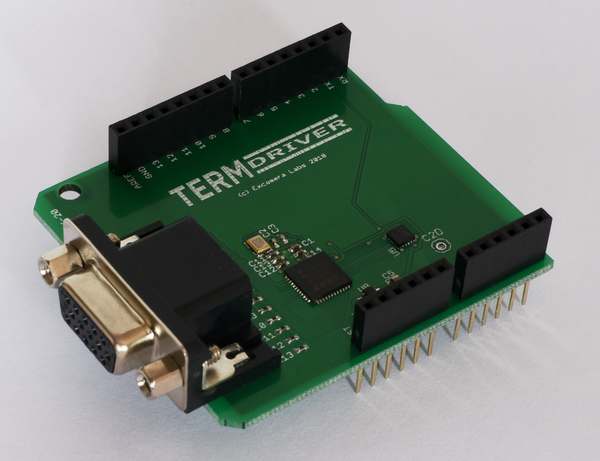
\includegraphics[width=0.75\textwidth]{img/img1}
  \caption{The TermDriver PCB}
\end{figure}

TermDriver listens on a serial line and emulates a text terminal on a
standard VGA connector. It gives embedded microcontrollers a real console.

\begin{itemize}
\item serial input at 115200 bps
\item connects to the Arduino serial output pin, no libraries required
\item supports standard ANSI terminal control codes
\item VGA 16-color output at 1024x768 
\item standard 80x25 and high-resolution 128x48 modes
\item rotated-screen 96x64 mode
\item screen-saver under CPU control
\item input signals 3.3V and 5V compatible
\end{itemize}

\newpage
\tableofcontents
\listoffigures

\newpage
\section{Installation with Arduino}

\begin{enumerate}
\item Disconnect power from the Arduino
\item Attach the TermDriver to the Arduino
\item Attach a VGA cable to the Arduino, turn on the VGA monitor
\item Apply power to the Arduino. You should see a blank screen with a blinking cursor at top-left
\item Load a sketch on the Arduino that prints text at 115200 baud, like the one below
\end{enumerate}

\newcommand{\eg}[1]{
\begin{framed}
\input{code/#1.inc}
\end{framed}
}

\eg{termdriver-helloworld}

\section{Operation}

\png{img/page1}{sample output at 80x25}

TermDriver monitors the serial line at 115200 baud, and draws any
text on the VGA.
There's nothing to set up or load.
For example this Arduino sketch

\eg{termdriver-counter1}

\noindent
Or this code in plain C

\eg{termdriver-counter2}

\noindent
Gives this output on the VGA:

\png{img/page2}{Counter output}

\subsection{ANSI escape codes}

The following standard
\href{https://en.wikipedia.org/wiki/ANSI_escape_code\#CSI_sequences}{CSI
codes} are supported:

\begin{longtable}[]{@{}ll@{}}
\toprule
\begin{minipage}[b]{0.34\columnwidth}\raggedright
Code\strut
\end{minipage} & \begin{minipage}[b]{0.60\columnwidth}\raggedright
Effect\strut
\end{minipage}\tabularnewline
\midrule
\endhead
\begin{minipage}[t]{0.34\columnwidth}\raggedright
ESC {[} \emph{n} A\strut
\end{minipage} & \begin{minipage}[t]{0.60\columnwidth}\raggedright
Cursor up\strut
\end{minipage}\tabularnewline
\begin{minipage}[t]{0.34\columnwidth}\raggedright
ESC {[} \emph{n} B\strut
\end{minipage} & \begin{minipage}[t]{0.60\columnwidth}\raggedright
Cursor down\strut
\end{minipage}\tabularnewline
\begin{minipage}[t]{0.34\columnwidth}\raggedright
ESC {[} \emph{n} C\strut
\end{minipage} & \begin{minipage}[t]{0.60\columnwidth}\raggedright
Cursor forward\strut
\end{minipage}\tabularnewline
\begin{minipage}[t]{0.34\columnwidth}\raggedright
ESC {[} \emph{n} D\strut
\end{minipage} & \begin{minipage}[t]{0.60\columnwidth}\raggedright
Cursor back\strut
\end{minipage}\tabularnewline
\begin{minipage}[t]{0.34\columnwidth}\raggedright
ESC {[} \emph{r;c} H\strut
\end{minipage} & \begin{minipage}[t]{0.60\columnwidth}\raggedright
Cursor position\strut
\end{minipage}\tabularnewline
\begin{minipage}[t]{0.34\columnwidth}\raggedright
ESC {[} \emph{n} J\strut
\end{minipage} & \begin{minipage}[t]{0.60\columnwidth}\raggedright
Erase display\strut
\end{minipage}\tabularnewline
\begin{minipage}[t]{0.34\columnwidth}\raggedright
ESC {[} \emph{n} m\strut
\end{minipage} & \begin{minipage}[t]{0.60\columnwidth}\raggedright
Select graphic rendition\strut
\end{minipage}\tabularnewline
\begin{minipage}[t]{0.34\columnwidth}\raggedright
ESC {[} s\strut
\end{minipage} & \begin{minipage}[t]{0.60\columnwidth}\raggedright
Save cursor position\strut
\end{minipage}\tabularnewline
\begin{minipage}[t]{0.34\columnwidth}\raggedright
ESC {[} u\strut
\end{minipage} & \begin{minipage}[t]{0.60\columnwidth}\raggedright
Restore cursor position\strut
\end{minipage}\tabularnewline
\bottomrule
\caption{this is a table}
\end{longtable}

In addition the following sequences are specific to TermDriver:

\begin{longtable}[]{@{}ll@{}}
\toprule
\begin{minipage}[b]{0.34\columnwidth}\raggedright
Code\strut
\end{minipage} & \begin{minipage}[b]{0.60\columnwidth}\raggedright
Effect\strut
\end{minipage}\tabularnewline
\midrule
\endhead
\begin{minipage}[t]{0.34\columnwidth}\raggedright
ESC {[} \emph{n} h\strut
\end{minipage} & \begin{minipage}[t]{0.60\columnwidth}\raggedright
Set display mode.

0 is 80x25, 1 is 128x48, 2 is 96x64 (rotated)\strut
\end{minipage}\tabularnewline
\begin{minipage}[t]{0.34\columnwidth}\raggedright
ESC {[} \emph{n} S\strut
\end{minipage} & \begin{minipage}[t]{0.60\columnwidth}\raggedright
Screen-saver.

0 stops video output, 1 restarts video output\strut
\end{minipage}\tabularnewline
\bottomrule
\caption{this is a table}
\end{longtable}

\subsection{High-resolution modes}

As well as the "classic" 80x25 text mode,
TermDriver also supports a higher density 128x48 mode,
and a portrait orientation 96x64 mode.
Both are very readable because
they match TermDriver's native 1024x768 @ 60 Hz VGA output.

\png{img/moby1}{mode 1: 128x48}
\png{img/moby2}{mode 2: 96x64}

\newpage
\section{Hardware}

\png{img/arduino}{Arduino Uno}

TermDriver connects directly to any Arduino or Arduino-compatible.
It uses four connections:

\begin{itemize}
\item \mach{GND}
\item \mach{5V}
\item \mach{RESET}
\item \mach{TX}
\end{itemize}

\noindent
To use any other MCU, make the above four connections. Note that RESET is active-high.
The serial protocol on \mach{TX} is 115200 bps, 8 bits, no parity, 1 stop bit.
This is frequently described as \mach{115200-8N1}.

\newpage
\hypertarget{technical-specifications}{}
\hypertarget{technical-specifications}{%
\section{Electrical characteristics}\label{electrical-characteristics}}

\subsection{DC characteristics}
\vspace{10 pt}
{\renewcommand{\arraystretch}{1.2}% for the vertical padding

\begin{tabularx}{\linewidth}{Xcccc}
\heavyline
& min & typ & max & units \\ \heavyline

Supply voltage & 4.0 & 5.0 & 9.0 & V \\ \hline

Supply current & & & & \\
\hspace{10pt} operating & & 25 & & mA \\
\hspace{10pt} screen saver & & 10 & & mA \\ \hline

RESET,RX low voltage & & & 0.6 & V \\ \hline
RESET,RX high voltage & 2.7 &   & 5.8 & V \\ \hline
\end{tabularx}}
\vspace{10 pt}

\subsection{AC characteristics}
\vspace{10 pt}

{\renewcommand{\arraystretch}{1.2}% for the vertical padding
\begin{tabularx}{\linewidth}{Xcccc}
\heavyline
& min & typ & max & units \\ \heavyline

Serial input line speed & & 115200 & & bps \\ \hline

VGA & & & & \\
\hspace{10pt} resolution & & 1024x768 & & pixels \\
\hspace{10pt} vertical sync & & 60.004 & & Hz \\
\hspace{10pt} horizontal sync & & 48.363 & & kHz \\
\hspace{10pt} pixel clock & & 65.000 & & MHz \\ \hline

Cursor blink rate & & 1.875 & & Hz \\ \hline
\end{tabularx}}
\vspace{10 pt}


\end{document}
